\chapter{Implementierung von Rayden}
\label{cha:Implementierung}

Diese Kapitel beschreibt die Implementierung von ausgewählten Komponenten des Rayden-System. Der Abschnitt \ref{cha:KeywordGrammar} zeigt die Grammatik und die \enword{Stack}-Maschine für die Ausführung von \enword{Keywords}. Es wird auf einzelne Implementierungsdetails detailliert eingegangen.  

\SuperPar
Im zweiten Abschnitt \ref{cha:Eval} wird der Aufbau von Ausdrücken beschrieben. Beendet wird dieser Abschnitt mit einem Auszug aus der \enword{RaydenExpressionEvaluator} Klasse, welche für die Auswertung der Ausdrücke zuständig ist. 

\SuperPar
Danach wird in Abschnitt \ref{cha:validateKeyword} die Validierung von Rayden-Tests gezeigt. Dafür wird das Validierungssystem von \enword{xText verwendet}. Abgeschlossen wird diese Kapitel mit dem Abschnitt \ref{cha:implementJSA}, welcher zeigt, wie die Integration des Rayden-Systems in das \enword{Java-Scripting-API} umgesetzt worden ist. 

%%------------------------------------------------------------------------------------------------------

\section{Umsetzung der \enword{Keyword}-Grammatik}
\label{cha:KeywordGrammar}

Die Rayden-Sprache wurde mit dem xText \cite{xtext} Compilerwerkzeug umgesetzt. Die Abbildung \ref{fig:keywordGrammar} zeigt einen Auszug aus der Grammatik für die Rayden-Sprache. Der Auszug zeigt die Grammatikregeln für \enword{Keywords}. Die Regel \enword{KeywordDecl} beginnt die Definition eines neuen \enword{Keywords}. Am Beginn der Regel wird der Typ für das \enword{Keyword} definiert. Eine Beschreibung und Auflistung der Typen ist in Abschnitt \ref{cha:KeywordTypes} enthalten. Danach folgt ein Name für das \enword{Keyword} welcher von einer öffneten geschwungenen Klammer gefolgt wird.

\begin{figure}
\centering
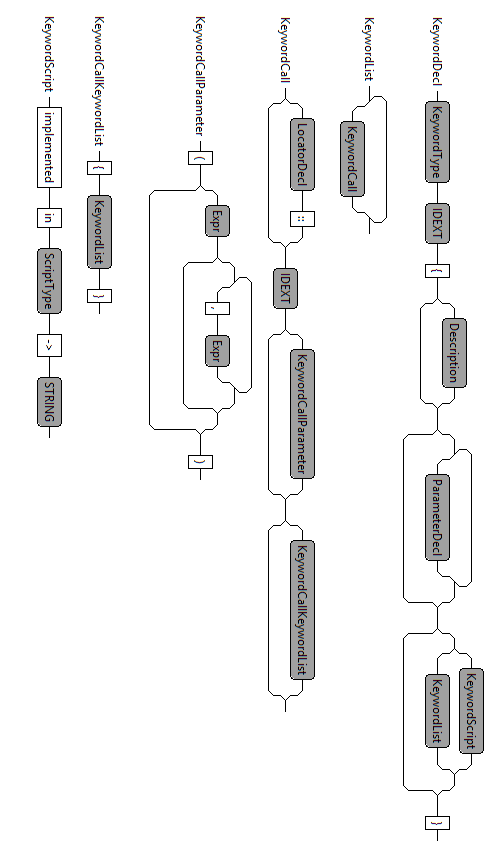
\includegraphics[width=0.9\textwidth]{grammar-keyword-all.png}
\caption{Auszug aus der Grammatik für \enword{Keywords}}
\label{fig:keywordGrammar}
\end{figure}

\SuperPar
Die geschwungenen Klammer definieren den Bereich der \enword{Keyword}-Implementierung. Am Anfang der Implementierung kann eine optionale Beschreibung angeführt werden. Diese wird von einer Parameterliste gefolgt. Ein Parameter wird mit der Regel \enword{ParameterDecl} beschrieben und kann 0 bis N Mal wiederholt werden. Eine Parameter-Definition besteht aus dem Schlüsselwort \enword{parameter}, einen Namen, einen Datentyp und einer Richtung.

\SuperPar
Danach folgt entweder die Bindung an ein Codestück mit der Regel \enword{KeywordScript} oder die \enword{Keyword}-Liste mit der Regel \enword{KeywordList} im Fall eines \enword{Compound-Keywords}. Die beiden Regeln sind wiederum optional um \enword{Keyword}-Rümpfe anlegen zu können. Diese Eigenschaft ist hilfreich, wenn die Testmanagerin oder der Testmanager nur die Struktur festlegen möchte, die Umsetzung des \enword{Keywords} jedoch von einem anderen Testpersonal vorgenommen wird. 

\begin{program}
\begin{JavaCode}
  Type Text (@PetClinic.PetClinicWeb.Login.Username , "max.mustermann")
	@PetClinic.PetClinicWeb.Login.Username :: Type Text ("max.mustermann")
	
	
	Click Left( @PetClinic.PetClinicWeb.Login.Go )
  @PetClinic.PetClinicWeb.Login.Go :: Click Left
\end{JavaCode}
\caption{Syntaktischer Zucker für die Verwendung von \enword{location}-Datentypen}
\label{prog:locatorSugar}
\end{program}

\SuperPar
Die Regel \enword{KeywordCall} definiert den Aufruf von einem \enword{Keyword} in einer \enword{Keyword}-Liste. Die Regel fängt normalerweise mit dem Namen des aufzurufenden \enword{Keywords} an. Danach folgt optional die Parameterliste für den Aufruf von dem \enword{Keyword}. Die Regel \enword{KeywrodCallParameter} definiert die Parameterliste, welche durch runde Klammer umschlossen ist. Die Parameter können als Liste von \enword{Expr}-Regeln definiert werden und werden durch einen Beistrich separiert werden. Für die einfachere Verwendung und besserer Lesbarkeit enthält die Regel \enword{KeywordCall} auch noch syntaktischen Zucker. Falls der erste Parameter von einem \enword{Keyword} vom Typen \enword{location} ist, kann diese Parameter vor das \enword{Keyword} geschrieben werden. Somit lässt sich die Implementierung leicht lesen. Der Codeausschnitt in Abbildung \ref{prog:locatorSugar} zeigt dazu die Verwendung des syntaktischen Zuckers im Vergleich zur klassischen Verwendung. Am Ende der \enword{KeywordCall}-Regel ist es noch möglich eine \enword{Keyword}-Liste zu definieren. Diese wird benötigt, falls es sich um ein \enword{Scripted-Compound-Keyword} oder um ein \enword{Inline-Keyword} handelt.

%%------------------------------------------------------------------------------------------------------

\section{Ausführung von \enword{Keywords} mit einer \enword{Stack}-Maschine}
\label{cha:StackMachine}

Im vorigen Abschnitt \ref{cha:KeywordGrammar} wurde die Grammatik von einem \enword{Keyword} in der Sprache Rayden erklärt. Dieser Abschnitt beschäftigt sich mit der Ausführung von \enword{Keywords}. Damit die \enword{Stack}-Maschine arbeiten kann, benötigt diese einen Zugriff auf den abstrakten Syntaxbaum. 

\begin{figure}
\centering
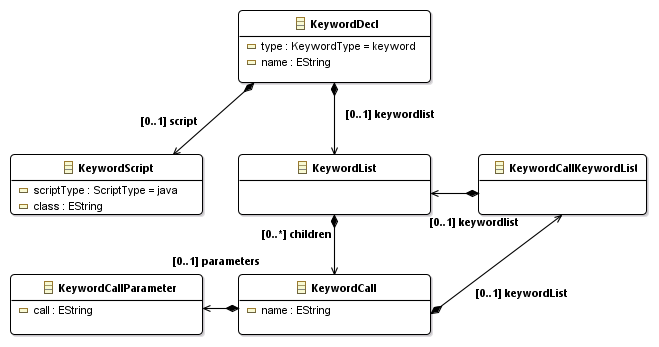
\includegraphics[width=1\textwidth]{keyword-model-diagramm.png}
\caption{Ausschnitt aus dem Abstrakte Syntaxbaum}
\label{fig:AST}
\end{figure}

\SuperPar
Das Compilerwerkzeug \enword{xText} stellt dafür ein \enword{Eclispe-ECore}-Modell zur Verfügung. Der generierten Compiler ist so konzipiert, dass dieser die gesamte Datei einliest und daraus einen abstrakten Syntaxbaum generiert. Der Syntaxbaum steht für die weitere Verarbeitung als \enword{ECore}-Modell zur Verfügung. Einen Auszug aus dem Modell zeigt die Abbildung \ref{fig:AST}. Die Abbildung zeigt die Modell-Repräsentation der Grammatik-Regeln von Abbildung \ref{fig:keywordGrammar}. Dieser Ausschnitt aus dem Modell stellt die Basis für die \enword{Stack}-Maschine dar. 

\SuperPar
Die \enword{Stack}-Maschine für das Rayden-System ist in der Klasse \enword{RaydenRuntime} implementiert. Der Codeauszug \ref{prog:runtime} zeigt die essentielle Methode \enword{executeKeyword}, welche für die Ausführung verantwortlich ist. Die Methode wird mit einem \enword{KeywordCall}-Objekt aufgerufen. Diese Objekt bezeichnet das erste \enword{Keyword}, welches von der \enword{Stack}-Maschine aufgerufen wird. Als erstes wird in der Methode übriggebliebene Element von dem \enword{Stack} entfernt. Danach wird über das \enword{Reporter-Interface} alle Objekte notifiziert, dass ein neuer Testfall gestartet worden ist. Im nächsten Schritt wird ein neuer Gültigkeitsbereich (\enword{RaydenScriptScope}) angelegt und mit dem \enword{KeywordCall}-Objekt initialisiert. Der Gültigkeitsbereich wird dann auf den leeren \enword{Stack} geladen. 

\SuperPar
Nach der Initialisierung der \enword{Stack}-Maschine wird die Abarbeitung gestartet. Es werden nun solange die Gültigkeitsbereiche am \enword{Stack} abgearbeitet, bis der \enword{Stack} leer ist oder ein Fehler bei der Ausführung von einem \enword{Keyword} aufgetreten ist. Der Gültigkeitsbereich repräsentiert einen Aufruf von einem \enword{Keyword} und die dazugehörigen Parameter und Variablen. Der Gültigkeitsbereich speichert zusätzlich die aktuelle Position in der \enword{Keyword}-Liste, falls es sich um ein \enword{Compound-Keyword} oder \enword{Scripted-Compound-Keyword} handelt. Über die Methode \enword{getNextOpt} kann die \enword{Stack}-Maschine das nächste \enword{Keyword} aus dem aktuellen Gültigkeitsbereich laden. Liefert die Methode kein Wert, ist die Ausführung des Gültigkeitsbereiches am Ende und wird daher vom \enword{Stack} entfernt.

\begin{program}
\lstinputlisting{samplecode/Runtime.java}
\caption{Codeauszug aus der \enword{RaydenRuntime}-Klasse}
\label{prog:runtime}
\end{program}

\SuperPar
Wurde jedoch ein Wert zurückgeliefert, wird mit der Ausführung fortgefahren. Handelt es sich bei dem Wert um ein \enword{KeywordCall}-Objekt, wird die Methode \enword{executeKeywordCall} aufgerufen. Diese Methode löst den Aufruf des \enword{Keywords} über eine \enword{Lookup}-Tabelle auf. Wurde die passende \enword{Keyword}-Implementierung gefunden, wird ein neuer Gültigkeitsbereich angelegt und auf den \enword{Stack} geladen. Wird in der \enword{Lookup}-Tabelle keine passende Implementierung gefunden, wird ein Fehler geworfen und die Ausführung abgebrochen. Handelt es sich jedoch um ein \enword{KeywordDecl}-Objekt wird das \enword{Keyword} ausgeführt.  

\SuperPar
Dabei muss die \enword{Stack}-Maschine überprüfen, ob es sich um ein \enword{Scripted-Compound-Keyword} handelt. Bei einem \enword{Scripted-Compound-Keyword} muss eine andere Logik ausgeführt werden, da es sowohl eine Code-Implementierung als auch eine \enword{Keyword}-Liste vorhanden ist. Bei allen anderen \enword{Keyword}-Metatypen wird die Methode \enword{executeKeywordDecl} ausgeführt. Diese Methode führt bei einem \enword{Scripted-Keyword} das spezifizierten Codestück aus. Bei einem \enword{Compound-Keyword} wird die \enword{Keyword}-Liste in den Gültigkeitsbereich geladen.

\SuperPar
Wurden alle Gültigkeitsbereich am \enword{Stack} erfolgreich abgearbeitet wird am Ende noch das \enword{Reporter-Interface} aufgerufen. Danach wird die Ausführung der \enword{Stack}-Maschine beendet.

%%------------------------------------------------------------------------------------------------------
\clearpage

\section{Auswertung von Ausdrücken}
\label{cha:Eval}

Dieser Abschnitt befasst sich mit den Grammatik-Regeln und der Ausführung von Ausdrücken. Die Rayden-Sprache unterstützt in einigen Bereichen der Sprache Ausdrücke. Ein Ausdruck kann in der Grammatik mit der Regel \enword{Expr} aufgerufen werden. Die Abbidlung \ref{fig:exprGrammar} zeigt einen Überblick über die Grammatik-Regeln von Ausdrücke. 

\begin{figure}
\centering
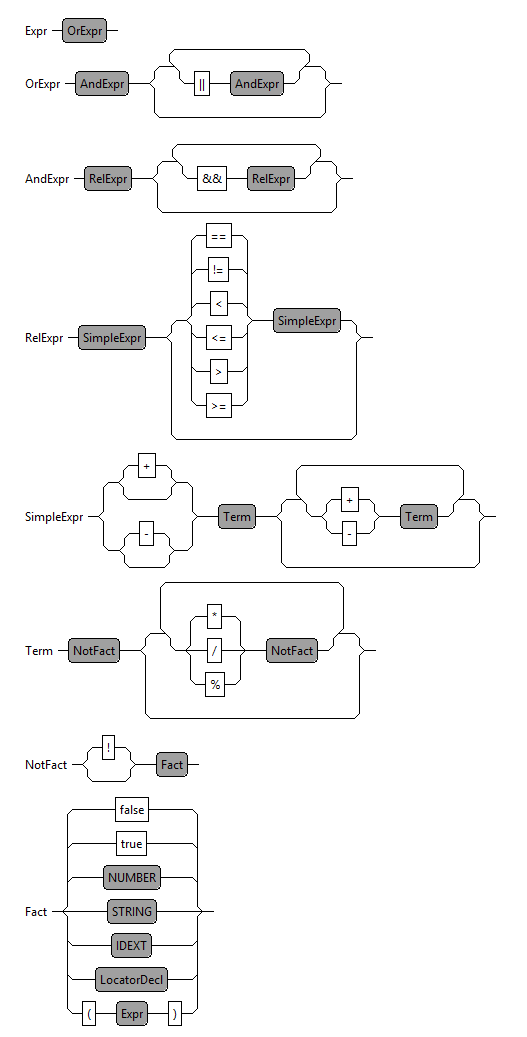
\includegraphics[width=0.9\textwidth]{grammar-expr.png}
\caption{Grammatik-Regeln für Ausdrücke}
\label{fig:exprGrammar}
\end{figure}

\SuperPar
Die Regeln für den Ausdruck sind klassisch aufgebaut. Die Operationen sind nach der Ausführungsreihenfolge in den Regeln eingearbeitet. Die am stärksten bindenden Operationen befinden sich in der Nähe der Blätter des Ausdrucksbaum. Die schwach bindenden Operationen befinden sich in der Nähe des Wurzelknotens. Die Blätter repräsentieren die Werte in einem Ausdruck, welche in der Regel \enword{Fact} definiert werden. Die Werte können entweder Konstanten oder Variablen sein und haben eine definierten Datentypen. Die Regel \enword{Fact} hat jedoch keinen spezielle Behandlung für \enword{Enumerations}. Der Grund dafür ist, dass \enword{Enumerations} intern als \enword{Strings} verarbeitet werden. Die Validierung der\enword{Enumerations} wird nur beim Initialisieren von Gültigkeitsbereichen durchgeführt.

\SuperPar
Für die Ausführung von Ausdrücken ist im Rayden-System die Klasse \enword{RaydenExpressionEvaluator} zuständig. Der Codeausschnitt \ref{prog:evaluator} zeigt eine Überblick über die Klasse \enword{RaydenExpressionEvaluator}. Die Klasse wird mit einem Gültigkeitsbereich initialisiert. Der Gültigkeitsbereich wird benötigt um Variablen bei der Abarbeitung auswerten zu können. 

\SuperPar
Die Auswertung eines Ausdrucks wird mit der Methode \enword{eval(Expr expression, String resultType)} gestartet. Als Parameter für die Methode wird ein \enword{Expr}-Objekt und eine Zeichenkette übergeben. Das \enword{Expr}-Objekt ist das Wurzelobjekt im \enword{ECore}-Modell für eine Ausdruck. Mit dem zweiten Parameter kann man die Auswertung des Ausdrucks typisieren. Wurde ein Typ definiert, wird am Ende der Auswertung noch überprüft, ob das Ergebnis vom selben Typ ist. Stimmt der Wert nicht überein, wird eine Fehler geworfen. Es gibt auch noch eine Spezialfall bei der Typisierung. Wird ein Ausdruck mit dem Typ \enword{variable} parametrisiert, werden keine Variablen im Ausdruck ausgewertet. Diese Eigenschaft wird benötigt, um Variablennamen an ein \enword{Keyword} übergeben zu können.

\SuperPar
Der Codeausschnitt \ref{prog:evaluator} enthählt am Ende die Implementierung der \enword{eval}-Methode für das Objekt \enword{Fact}. Diese Methode zeigt, wie die Werte aus dem \enword{ECore}-Modell nach \enword{Java} konvertiert werden. Die Methode zeigt auch, wie Variablen mithilfe des Gültigkeitsbereichs ausgewertet werden können.

\begin{program}
\lstinputlisting{samplecode/RaydenExpressionEvaluator.java}
\caption{Codeauszug aus dem \enword{RaydenExpressionEvaluator}}
\label{prog:evaluator}
\end{program}

%%------------------------------------------------------------------------------------------------------
\clearpage
\section{Überprüfung der \enword{Keyword}-Referenzen}
\label{cha:validateKeyword}

\begin{program}
\lstinputlisting{samplecode/Validator.java}
\caption{Codeauszug aus dem \enword{RaydenDSLJavaValidator}}
\label{prog:validator}
\end{program}

%%------------------------------------------------------------------------------------------------------

\section{Implementierung der \enword{Java-Scripting-API}}
\label{cha:implementJSA}

\begin{program}
\lstinputlisting{samplecode/ScriptEngine.java}
\caption{Codeauszug aus der \enword{RaydenScriptEngine}}
\label{prog:scriptEngine}
\end{program}

\todo

